\documentclass[11pt,a4paper]{article}
\usepackage[T1]{fontenc}
\usepackage[utf8]{inputenc}
\usepackage{mathptmx}
\usepackage[margin=2.35cm]{geometry}
\usepackage{graphicx}
\usepackage{amsmath}
\usepackage{booktabs}
\usepackage{microtype}
\usepackage{caption}
\usepackage{titlesec}
\usepackage[hidelinks]{hyperref}
\usepackage{xurl}
\usepackage{placeins}
\captionsetup{font=small,labelfont=bf}
\titleformat{\section}{\normalfont\large\bfseries}{\thesection.}{0.6em}{}
\titleformat{\subsection}{\normalfont\normalsize\bfseries}{\thesubsection}{0.6em}{}
\titlespacing{\section}{0pt}{1.1em}{0.4em}
\setlength{\parskip}{2pt}
\newenvironment{apabib}{\raggedright\begin{list}{}{%
  \setlength{\leftmargin}{1.6em}\setlength{\itemindent}{-1.6em}%
  \setlength{\itemsep}{3pt}\setlength{\parsep}{0pt}\setlength{\topsep}{4pt}}}%
  {\end{list}}
\newcommand{\Clm}{\mathrm{Cl}^{-}}
\newcommand{\ECl}{E_{\mathrm{Cl}}}

\title{\vspace{-1.6em}\textbf{From homeostasis to computation:\\[2pt]
could the GABA switch build the core of the signed-XOR motif?}}

\author{Jes\'us Marco de Lucas\\[2pt]
\small Instituto de F\'isica de Cantabria (IFCA), CSIC--Universidad de Cantabria, Santander, Spain\\
\small \texttt{marco@ifca.unican.es} \quad ORCID:~0000-0001-7914-8494}
\date{\small \textsc{Hypothesis and Theory Article} \\ Draft --- July 2026}

\begin{document}
\maketitle
\vspace{-1.4em}

\begin{abstract}\noindent
We have proposed the \emph{signed-XOR mechanism}, a feedforward-inhibition motif whose common, shunting hub computes at once an XOR-type gate and emits a local \emph{signed} error, as a recurrent connectomic motif (Pe\~na Fern\'andez et al., 2026a), as a computational primitive (2026b), and as relevant for memory (2026c). In trying to understand why inhibitory neurons are so central in the hippocampus, a key site for memory, we were struck by the developmental ``GABA switch'': the same inhibition that is depolarizing and \emph{network-building} in the early vertebrate brain becomes shunting and \emph{computation-controlling} upon maturation, when the chloride extruder KCC2 lowers intracellular chloride in the neurons and reverses the sign of the GABA driving force. This note asks whether that switch could help to explain how a motif as intricate as the signed-XOR, an inhibitory hub that must sit at the centre of the excitatory arms it regulates, flanked by two opponent output channels, could \emph{emerge}. We develop a single, deliberately speculative thesis: \emph{computation is repurposed homeostasis}. 
We make the idea concrete in two conductance-based simulations: a single moving reversal potential flips a network from a synchronous builder to a stable governor, and, given a pre-positioned shunting hub, calcium-dependent
plasticity grows the input-to-lateral arms into an XOR-like read-out, thereby forming the coincidence-suppression core of the motif, with the shunt acting at once as the mature operation and as the teaching signal.
The chloride-controlled sign of GABA turns out to run deeper than vertebrate development --- it is conserved down to \emph{C.~elegans}, though the worm shows the switch, not the computational motif --- while the molecular kit of such a shunting governor is in fact pre-neuronal: plants already use it for turgor and movement. What animals add is the active \emph{extrusion} of chloride, which turns a depolarizing anionic signal (movement-like) into a shunting one (control-like), providing one route by which homeostatic regulation could acquire a computational role.
\end{abstract}

\noindent\textbf{Keywords:} signed-XOR motif; chloride homeostasis; GABA switch; KCC2/NKCC1; shunting inhibition; divisive normalization; BCM; predictive coding; evolution of computation.

\section{Introduction}\label{sec:intro}

We have argued in a series of recent contributions that a small, concrete circuit, the \emph{signed-XOR mechanism}, recurs in many connectomes and is a natural unit of neural computation: we introduced this motif as an over-represented connectomic pattern for local directional error signalling (Pe\~na Fern\'andez et al., 2026a), framed its XOR operation as a neuronal loss function and computational primitive (Pe\~na Fern\'andez et al., 2026b), and related it to memory (Pe\~na Fern\'andez et al., 2026c). In this motif, two inputs each excite a ``lateral'' principal cell and, in parallel, a common inhibitory \emph{hub}; the hub returns \emph{shunting} (divisive) inhibition to these laterals, so that a read-out pooling them responds strongly to a single input but is suppressed when both coincide, implementing an XOR-type gate, categorical once a downstream firing threshold is applied. Two aggregators of \emph{opposite neurotransmitter identity}, $F^{+}$ and $F^{-}$, read the circuit as a local \emph{signed} error $e=F^{+}-F^{-}$, precisely the quantity a backpropagation-free learning rule needs.  

This note takes a different perspective. In trying to understand \emph{why} inhibitory neurons should be so central in the hippocampus, a key site for memory, we arrived at a developmental fact that is well known but, in this context, striking: the \emph{GABA switch}. Early in the development of neural circuits, GABA does not act as an inhibitory neurotransmitter but as a \emph{depolarizing}, network-recruiting one (depolarizing, and under the right conditions excitatory). We suggest that the same interneurons that will later regulate the network may first help to \emph{build} it; only when the chloride extruder KCC2 matures does intracellular chloride fall, the GABA reversal potential drop towards rest, and the very same inhibitory conductance shift from a depolarizing builder to a shunting governor. One conductance; two opposite computational roles, selected by a single homeostatic set point.

This duality is suggestive, because the signed-XOR motif is itself hard to specify from scratch: an inhibitory element that must occupy the centre of a convergent excitatory circuit, flanked by two output channels of opposite sign. Could the same switch that flips inhibition from builder to governor also help to explain how such a motif \emph{emerges}? 

We develop a speculative thesis: \emph{computation is repurposed homeostasis}, as the acquisition of active chloride extrusion turns an ancient anionic turgor/movement signal, already present in plants\footnote{A clear caveat: the plant and animal molecules involved are \emph{not} homologous; this is functional repurposing of an ancient ion-control principle, not shared ancestry.}, into a shunting feedback governor, and the signed-XOR mechanism is where that governor is housed.  

To provide a visual scheme of the idea to the interested reader, the mature topology and operations of the motif are shown in Fig.~\ref{fig:mature}, while the two developmental steps that build it thanks to the GABA switch are sketched in Fig.~\ref{fig:devseq}.


\begin{figure}[t]
\centering
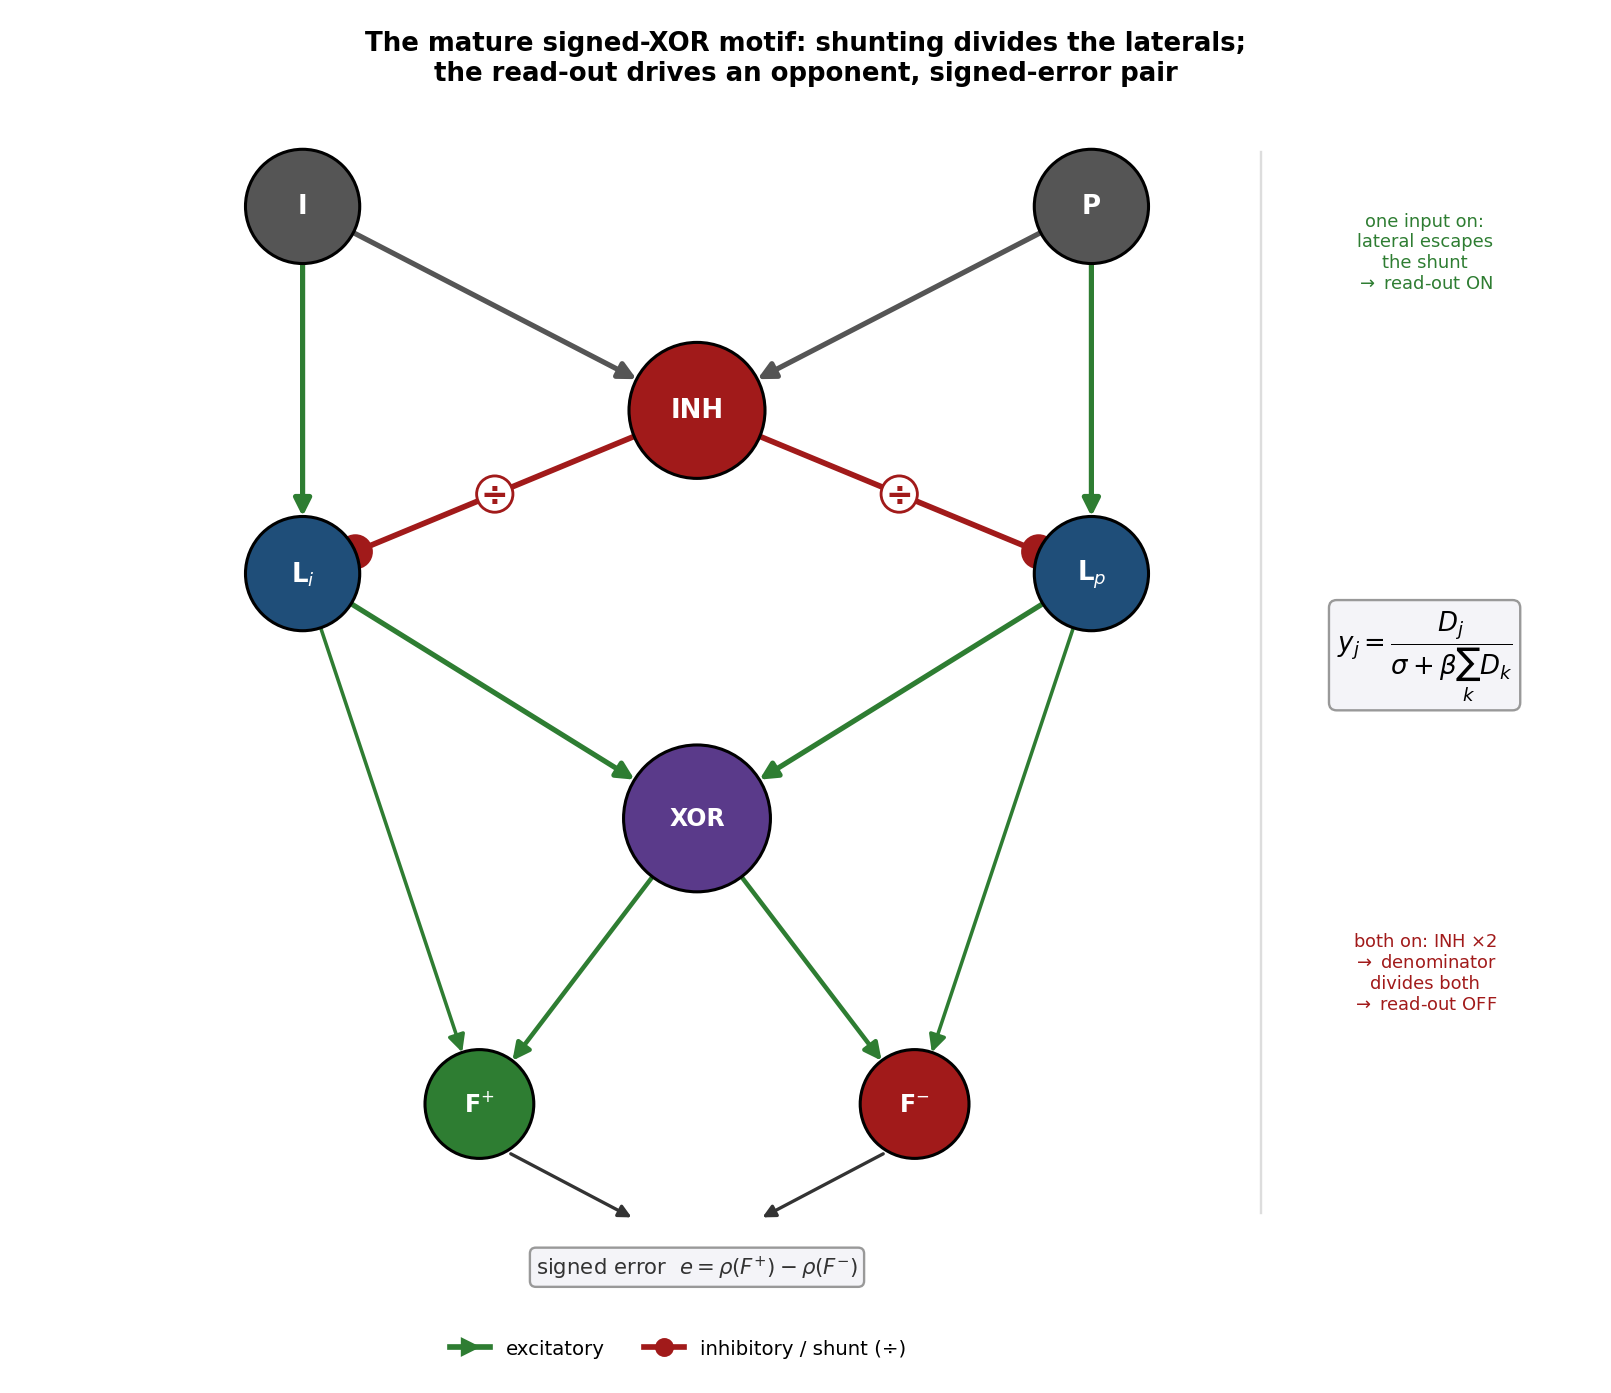
\includegraphics[width=0.66\linewidth]{motif_mature_en.png}
\caption{\textbf{The mature signed-XOR motif and its operations.} Each input excites its lateral and, in parallel, the common hub, which returns shunting inhibition ($\div$) only to the two laterals. A single input leaves the hub barely recruited, so its lateral escapes the shunt (read-out ON); two inputs recruit the hub \emph{supralinearly}, so that the denominator grows faster than the drive and divides both laterals down (read-out OFF) --- a soft XOR-type gate that a downstream firing threshold makes categorical. The read-out projects to both aggregators, and each lateral to one of them ($L_i\!\to\!F^{+}$, $L_p\!\to\!F^{-}$); the two aggregators have opposite neurotransmitter identity, and their difference is the local signed error $e=\rho(F^{+})-\rho(F^{-})$.}
\label{fig:mature}
\end{figure}

\begin{figure}[t]
\centering
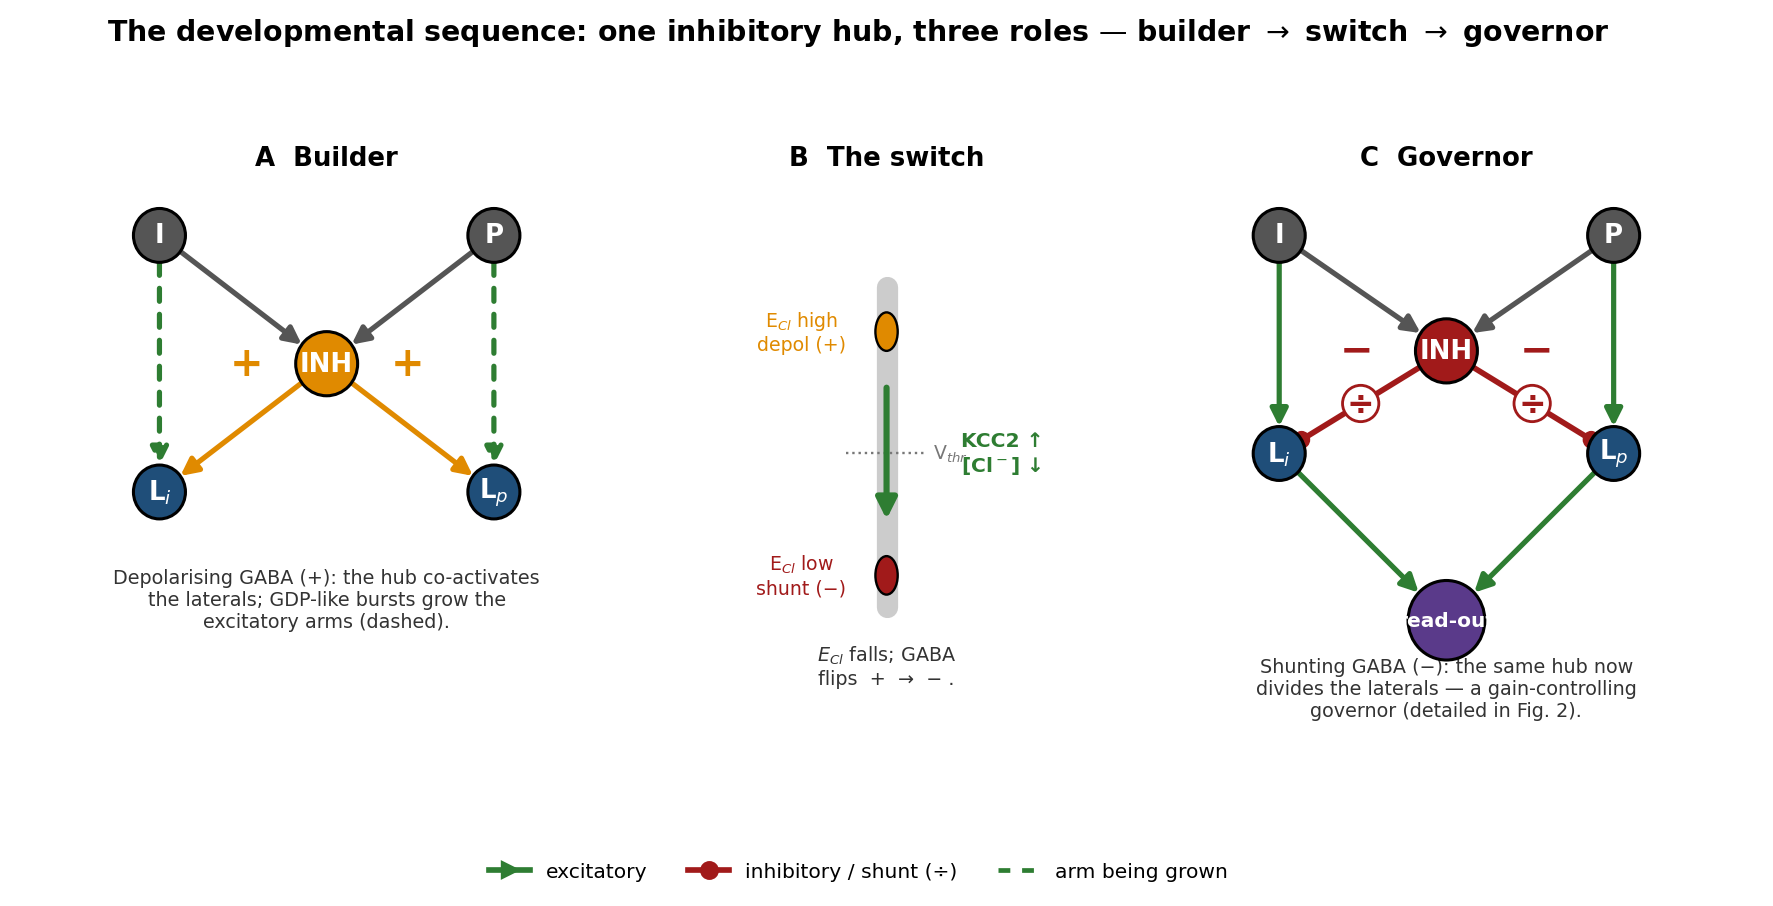
\includegraphics[width=\linewidth]{motif_dev_en.png}
\caption{\textbf{The developmental sequence: one inhibitory hub, three roles.} \textbf{(A) Builder.} While intracellular chloride is high, GABA is depolarizing ($+$) and the hub coactivates (recruits) the laterals $L_i,L_p$; GDP-like bursts grow the excitatory input arms (dashed). \textbf{(B) The switch.} As KCC2 rises and chloride falls \emph{in the lateral (postsynaptic) cells}, their GABA reversal potential $\ECl$ drops from above the firing threshold towards rest, so that the hub's synapses onto them shift from depolarizing ($+$) to shunting ($-$). \textbf{(C) Governor.} The same hub, now central, \emph{shunts} ($\div$) the laterals, becoming a gain-control governor whose mature circuit and operations are detailed in Fig.~\ref{fig:mature}. Excitatory connections end in arrowheads; shunting ones, in filled circles.}
\label{fig:devseq}
\end{figure}

The following sections state the argument compactly; the results of the simulations and the supporting biology can be found in Appendices~\ref{app:sim}--\ref{app:plants}.

\section{The GABA switch and the motif it could implement}\label{sec:switch}
The GABA switch is a single change in the neurons that receive GABA: GABA$_{\mathrm{A}}$ receptors open a chloride channel, so that its reversal potential $\ECl$ is set by intracellular chloride in the postsynaptic cell, which the cotransporters actively control; NKCC1 imports chloride ($\ECl$ high, GABA depolarizing), KCC2 extrudes it ($\ECl$ low, GABA shunting). Neurons express NKCC1 early and KCC2 late, so that GABA begins depolarizing and ends shunting, as has been observed in the hippocampus (Appendix~\ref{app:hipp}), but also in \emph{C.~elegans} (Appendix~\ref{app:worm}). This set point is not merely developmental drift: it is under active homeostatic control. The WNK--SPAK/OSR1 kinase cascade reciprocally regulates the two cotransporters, activating NKCC1 while inhibiting KCC2, and WNK itself senses intracellular chloride, so that the very variable that decides whether GABA recruits or shunts sits inside a molecular feedback loop (Appendix~\ref{app:bg}). Notice that the inhibitory \emph{conductance} is present the whole time; only the sign of its driving force changes.

In its depolarizing phase an interneuronal hub \emph{coactivates} its targets and paces the synchronous bursts known as giant depolarizing potentials (GDPs), whose calcium transients grow the excitatory arms: the hub literally helps to build the circuit it will later regulate, and GABAergic \emph{hub} interneurons are known to orchestrate exactly this early synchrony (Bonifazi et al., 2009). After the GABA switch, the same hub, now central, \emph{shunts} those targets: it becomes a divisive gain controller. We call these two modes \emph{builder} and \emph{governor} (Fig.~\ref{fig:devseq}, Appendix~\ref{app:hipp}).

The hardest question is topological: why should the inhibitory hub come to sit at the centre of the excitatory arms, wired so as to \emph{suppress} coincidence? Correlation-based growth cannot do it: ``neurons that fire together wire together'' reinforces coincidence, which is exactly the opposite of what an XOR-type gate requires. But the switch supplies the missing, symmetry-breaking signal. Development hands us a pre-positioned, broadly connected inhibitory hub (Fig.~\ref{fig:devseq}A); once that hub shunts, ordinary calcium-dependent plasticity does the rest. A lateral driven by a \emph{single} input escapes the shunt, depolarizes, admits a large calcium transient and \emph{potentiates} its arm; a lateral driven during \emph{coincidence} is clamped by the doubled shunt, its calcium collapses, and its arm \emph{depresses}. The shunt is at once the mature operation \emph{and} the teaching signal that carves it.

Two conditions must hold for this to converge, and we state both as predictions. First, the common shunt onto a lateral must be \emph{supralinear} in the number of coincident inputs, $g_{\mathrm{inh}}(2)>2\,g_{\mathrm{inh}}(1)$, so that a single input barely activates it while a coincident pair clamps the lateral hard; in our model this supralinearity comes from the hub's own firing threshold, that is, from interneuron recruitment, amplified by the voltage dependence of calcium entry. Second, the arms must \emph{clear} the firing ``cliff'', where a single input drives the lateral --- but this need not be assumed: the depolarizing \emph{builder} phase lifts them there (Appendix~\ref{app:sim}). Conductance-based simulations confirm that the full builder$\to$switch$\to$governor sequence suffices, and that deleting any one phase abolishes the result; remove the hub and the identical rule gives OR. The wiring, in short, need not be specified synapse by synapse. It is the fixed point of ordinary plasticity operating under a pre-positioned shunt.

\section{Emergence of the signed-XOR as a computational motif}\label{sec:compute}
What development leaves behind is a topology, not yet a computation. What converts one into the other is the shunt, in a chain of four steps worth keeping distinct. \emph{(i)}~A common conductance-based inhibitor produces \emph{shunting} inhibition (\S\ref{app:bg}). \emph{(ii)}~Shunting implements \emph{divisive gain control}, divisive normalization in the canonical sense (Carandini \& Heeger, 2012): the excitatory drive $D_i$ to a lateral is divided by a denominator that grows with the shunt the hub returns. Writing $g$ for the hub's recruitment, the read-out of lateral $i$ is
\begin{equation}
y_i \;=\; \frac{D_i}{\sigma \;+\; \beta\, g\!\left(\textstyle\sum_{k} D_k\right)},
\end{equation}
the common shunt sitting in the denominator (Fig.~\ref{fig:mature}, where the hub shunts the laterals, marked $\div$). \emph{(iii)}~Coincidence is suppressed only if that denominator grows \emph{faster} than the drive. This is the crux, and it is worth being explicit, because a \emph{linear} pool ($g(x)=x$) does not suffice: with one input, $y_{10}=D/(\sigma+\beta D)$; with two, $y_{11}=2D/(\sigma+2\beta D)$, and $y_{11}/y_{10}=2(\sigma+\beta D)/(\sigma+2\beta D)>1$ for any $\sigma>0$. Linear divisive normalization can \emph{saturate} the pooled read-out but cannot invert it: it yields gain control, not XOR. Coincidence suppression requires the shunt recruitment to be \emph{supralinear}, $g(2D)>2\,g(D)$, and specifically
\begin{equation}
\beta\,\big[\,g(2D) - 2\,g(D)\,\big] \;>\; \sigma,
\label{eq:xorcond}
\end{equation}
so that doubling the input more than doubles the denominator and drives both laterals down (read-out OFF), while a single input leaves the shunt barely recruited (read-out ON). \emph{(iv)}~This coincidence suppression becomes an \emph{XOR-type} operation only after thresholding: a firing threshold $z=H(y-\vartheta)$ ($H$ the Heaviside step) turns the graded preference into a categorical exactly-one.

We claim \emph{only} this chain, supralinear shunting $\to$ coincidence suppression $\to$ thresholded XOR, and \emph{not} a Boolean XOR at the biophysical level: the gate is graded (in our simulations, single-input drive exceeds coincident drive several-fold, not infinitely), so that ``exactly-one'' always refers to the thresholded read-out. The supralinearity is not an extra assumption bolted on for this section; it is the same condition the growth model needs to converge (\S\ref{sec:switch}), and in the circuit it comes from the hub's own firing threshold --- interneuron recruitment --- amplified by the voltage dependence of calcium entry.

Divisive normalization is, however, a waypoint and not the destination. It is a canonical cortical operation, found almost everywhere it has been looked for, and on its own it buys us nothing new: a gain-control circuit is not yet a computational motif. What makes this one a motif is what reads it. Two aggregators of \emph{opposite neurotransmitter identity}, $F^{+}$ (excitatory) and $F^{-}$ (inhibitory), pool the circuit, and their difference
\begin{equation}
e \;=\; \rho(F^{+}) - \rho(F^{-}),
\end{equation}
with $\rho$ a non-negative activation, is a local \emph{signed} error.

The sign is the whole point, and it is what the bare gate cannot give. A thresholded XOR reports only \emph{that} the two inputs disagree; it is a magnitude without a direction. The opponent pair recovers the direction, because the read-out projects to both aggregators while each lateral projects to one of them ($L_i\!\to\!F^{+}$, $L_p\!\to\!F^{-}$), so that the residual difference carries not just the mismatch but its polarity. That is precisely the quantity a backpropagation-free learning rule needs, and the one that schemes such as equilibrium propagation (Scellier \& Bengio, 2017) and predictive coding (Whittington \& Bogacz, 2017) construct by other means; it is also the role we have argued the motif plays in local credit assignment (Pe\~na Fern\'andez et al., 2026a) and as a neuronal loss function (2026b).

Nor need the error be transported anywhere. In the most local reading, $F^{+}$ and $F^{-}$ are opposite excitatory and inhibitory feedback synapses onto the same postsynaptic compartment, so that their difference is simply the local depolarization there, which through the calcium code sets postsynaptic calcium and hence the sign of plasticity (Appendix~\ref{app:sim}). The signed-XOR motif, on this reading, is not a gate that happens to compute XOR. It is an error-generating element, and the gate is what makes its error informative.

\section{An evolutionary reading}\label{sec:evo}

The materials used are ancient and widespread: plants also use chloride and anion channels to drive turgor and movement, and even use GABA to modulate anion channels, but they keep chloride \emph{high} and never acquire an animal-style plasma-membrane extrusion regime, so that they have the ancient ingredients without the one specialization that makes GABA shunting (Appendix~\ref{app:plants}). On this reading, the GABA switch is the animal innovation that turns movement into control.

Read broadly, the switch is an instance of a general move. \emph{Homeostasis} keeps the conditions for life; \emph{control} is homeostasis with feedback; and the minimal feedback element in an excitable membrane is a \emph{shunt}, a conductance that lowers the input resistance and so divisively attenuates other inputs. Acquiring active chloride extrusion is what turns an anionic movement/turgor signal into a computational feedback governor, by setting the anionic driving force near rest so that the conductance shunts rather than drives. The extrusion machinery --- the cation-chloride cotransporter family --- long predates neurons (Hartmann et al., 2014); nervous systems plausibly arose to coordinate contractile and ciliary effectors (Keijzer et al., 2013; J\'ekely et al., 2015), so that the appearance of the chloride switch even in the \emph{muscle} of \emph{C.~elegans} fits a picture of shunting control as a general tool of the excitable cell, deployed in muscle for movement and in neurons for computation. Plants provide an informative functional contrast: they use chloride, anion channels, GABA-related signalling, and turgor-based excitability, but they do not deploy an animal-style plasma-membrane chloride-extrusion regime to make GABA shunting. The parallel is convergent, not homologous --- the conserved threads are the ancient cotransporter family and the \emph{strategy} of using an anionic conductance to set excitability, not a shared receptor.

\section{Predictions and caveats}\label{sec:pred}
\textbf{Predictions.} Manipulating the chloride extruders (KCC2/ABTS-1) should degrade \emph{both} the \emph{stabilizing} and the \emph{XOR-computing} functions at once, since they are the same shunt; strong recurrent excitation \emph{before} the switch should give runaway epileptiform dynamics rather than computation; the inhibitory hub of a signed-XOR circuit should be early-maturing and broadly connected, and its shunt \emph{supralinear} in the number of coincident inputs (a condition our simulations needed in order to converge); and blocking coincidence-induced postsynaptic calcium suppression during development should push the emergent XOR read-out towards OR.

\textbf{Caveats.} The biology of each layer is established; the \emph{unifying} claim --- a single governor repurposed from homeostasis to computation, and specifically the signed-XOR motif --- is an interpretive hypothesis, not a result. The hypothesis addresses, strictly, the emergence of the shunting \emph{coincidence-suppression core}: the pre-positioned inhibitory hub and the supralinear shunt that carves an XOR-type read-out. It does \emph{not} explain the origin of the opponent read-out channels $F^{+}$ and $F^{-}$ --- why they should appear, why with opposite neurotransmitter identity, or why each lateral should project selectively to one of them. Those are taken here as part of the mature signed-XOR architecture proposed previously (Pe\~na Fern\'andez et al., 2026a,b); how the opponent pair itself develops remains an additional and unsolved problem. The plant/animal parallel is convergent. The worm's switch is largely cell-intrinsic, so that the activity-dependent, self-organizing version is a vertebrate elaboration, not a universal. The XOR is soft, not exact. And the growth model is a proof of principle with the limits set out in Appendix~\ref{app:sim}. We have tried to keep the established visibly separate from the speculative.

\section{Conclusion}\label{sec:concl}
The ingredients of a computational feedback element --- chloride, anion channels, GABA, and the cotransporters that set the chloride gradient --- are older than neurons and are already, in plants, the machinery of turgor and movement. What animals add is active chloride extrusion, which reverses the sign of the anionic driving force and turns a movement-like signal into a shunting, gain-controlling one. On this reading, the developmental GABA switch is not a curiosity of hippocampal wiring, but a route by which an inhibitory hub is repurposed from builder to governor --- and, we suggest, by which a motif as intricate as the signed-XOR could \emph{emerge}, grown by the very shunt with which it will compute. We offer the synthesis as a target: to sharpen it, test it, and, where needed, knock it down.

\vspace{0.4em}
\noindent\textbf{Data and code.} The simulations (the GABA switch and the BCM-guided signed-XOR growth) are released at \url{https://github.com/[to-be-completed]/EmergingXOR} and will accompany the published article.

\vspace{0.2em}
\noindent\textbf{Competing interests.} The author declares a competing interest: a related European patent application, \emph{Signed XOR Feedback} (No.~26382252.0), has been filed (Marco de Lucas et al., 2026).

% ============================== APPENDICES ==============================
\FloatBarrier
\appendix
\titleformat{\section}{\normalfont\large\bfseries}{Appendix~\thesection.}{0.6em}{}
\titlespacing{\section}{0pt}{1.2em}{0.4em}


\section{Background biophysics, minimal simulations, and code}\label{app:sim}
\subsection{Background: driving forces, shunts, and the calcium code}\label{app:bg}

\textbf{(i) Driving force.} A neuron's membrane holds a voltage $V$; each ion has an equilibrium (reversal) potential $E_{\mathrm{ion}}$, and the current through an open channel is the conductance $g$ times the driving force $(V-E_{\mathrm{ion}})$, that is, $I = g\,(V - E_{\mathrm{ion}})$. 
Opening a channel pushes $V$ towards $E_{\mathrm{ion}}$ \emph{and} lowers the input resistance (a ``shunt''). When $E_{\mathrm{ion}}$ is well below rest, the channel hyperpolarizes (subtractive inhibition); when $E_{\mathrm{ion}}$ is \emph{near} rest, it barely changes $V$ but still adds conductance, so that it mostly \emph{divides} other inputs, shunting (divisive) inhibition, the substrate of gain control (Carandini \& Heeger, 2012). The same channel can be excitatory, shunting, or hyperpolarizing depending only on where $E_{\mathrm{ion}}$ sits relative to $V$.

\textbf{(ii) The chloride machinery.} GABA$_{\mathrm{A}}$ receptors open a chloride channel, so that their reversal potential is essentially $\ECl$, set by $[\Clm]_{\mathrm{in}}$. Concretely, because the open GABA$_{\mathrm{A}}$ channel is chloride-selective, $\ECl$ follows the Nernst relation
\begin{equation}
\ECl \;=\; \frac{RT}{z_{\Clm}F}\,\ln\frac{[\Clm]_{\mathrm{out}}}{[\Clm]_{\mathrm{in}}}
     \;=\; \frac{RT}{F}\,\ln\frac{[\Clm]_{\mathrm{in}}}{[\Clm]_{\mathrm{out}}},
\end{equation}
with valence $z_{\Clm}=-1$ for the anion; the sign is the point --- opposite to a cation, \emph{raising} intracellular chloride moves $\ECl$ to more depolarized values (builder), while lowering it drags $\ECl$ towards rest (governor). The importer NKCC1 raises $[\Clm]_{\mathrm{in}}$ (pushing $\ECl$ above rest); the extruder KCC2 lowers it (dragging $\ECl$ towards rest). Immature neurons express NKCC1 early and KCC2 late, so that GABA depolarizes early and shunts late. The \emph{GABA switch} is not a change of transmitter or receptor, but of a single homeostatic set point, $[\Clm]_{\mathrm{in}}$.

It is worth being explicit about \emph{why} these two proteins can hold such different set points, because the answer is pure thermodynamics rather than biological detail. Both are electroneutral cotransporters --- NKCC1 carries 1\,Na$^{+}$:1\,K$^{+}$:2\,$\Clm$, KCC2 carries 1\,K$^{+}$:1\,$\Clm$ --- so no net charge crosses the membrane and the free energy of transport contains no $zF\Delta\psi$ term. Direction is set by chemical potentials alone, and each transporter therefore has a hard equilibrium condition. KCC2 runs until $[\mathrm{K}^{+}]_{\mathrm{in}}[\Clm]_{\mathrm{in}}=[\mathrm{K}^{+}]_{\mathrm{out}}[\Clm]_{\mathrm{out}}$, that is, until $\ECl\rightarrow E_{\mathrm{K}}\approx-90$~mV. NKCC1 runs until $[\mathrm{Na}^{+}]_{\mathrm{in}}[\mathrm{K}^{+}]_{\mathrm{in}}[\Clm]_{\mathrm{in}}^{2}=[\mathrm{Na}^{+}]_{\mathrm{out}}[\mathrm{K}^{+}]_{\mathrm{out}}[\Clm]_{\mathrm{out}}^{2}$, that is, until $\ECl\rightarrow(E_{\mathrm{Na}}+E_{\mathrm{K}})/2\approx-15$~mV. The two transporters pull $\ECl$ towards attractors some 75~mV apart, and the neuron's actual $\ECl$ settles wherever their relative fluxes --- together with the GABA$_{\mathrm{A}}$ and leak conductances --- balance. The developmental switch is not a change of mechanism at all: it is a change in which attractor wins.

\textbf{(iii) Who moves the set point: the WNK--SPAK chloride thermostat.} The set point is not merely a passive consequence of gene expression; it is the output of a genuine homeostatic controller, and this is the level at which the ``computation is repurposed homeostasis'' thesis is most literal. The large cytoplasmic C-terminal domains of both cotransporters carry the phosphosites of the WNK--SPAK/OSR1 kinase cascade, and the cascade acts on them with \emph{opposite sign}: phosphorylation by SPAK/OSR1 activates NKCC1 and inhibits KCC2, while dephosphorylation does the reverse, so that a single kinase reciprocally sets the balance of import and extrusion (Rinehart et al., 2009). The two inhibitory threonines of KCC2, Thr906 and Thr1007, are highly phosphorylated in immature neurons and are progressively dephosphorylated as they mature; blocking or depleting WNK1 in immature neurons is by itself enough to enhance chloride extrusion and shift $E_{\mathrm{GABA}}$ towards hyperpolarizing values (Friedel et al., 2015). The loop closes because WNK is itself a \emph{chloride sensor}: $\Clm$ binds directly in the catalytic site and stabilizes the inactive conformation, inhibiting autophosphorylation (Piala et al., 2014). Low $[\Clm]_{\mathrm{in}}$ therefore activates WNK, which switches NKCC1 on and KCC2 off, and chloride rises; high $[\Clm]_{\mathrm{in}}$ inhibits WNK and the reverse occurs. Sensor, comparator and reciprocal actuators are all molecular, and together they implement a negative-feedback loop --- a chloride thermostat --- whose set point is exactly the variable that decides whether the inhibitory hub of the motif is a builder or a governor. On this reading the GABA switch is not a developmental accident overlaid on a computing circuit; it is a homeostatic controller being re-tuned, and the computation is what that re-tuning leaves behind.

\textbf{(iv) The calcium code.} Whether a synapse potentiates (LTP) or depresses (LTD) is governed, to good approximation, by postsynaptic calcium, which enters through voltage-dependent routes (NMDA receptors, voltage-dependent calcium channels) and therefore tracks how strongly the cell depolarized: \emph{moderate} calcium induces LTD, \emph{high} calcium LTP (Graupner \& Brunel, 2012; Clopath et al., 2010). The Bienenstock--Cooper--Munro (BCM) theory adds a \emph{sliding} threshold that follows the neuron's own recent activity, stabilizing the loop (Bienenstock et al., 1982). The consequence this note exploits: because calcium entry is voltage-dependent and a shunt limits depolarization, a shunting hub controls the postsynaptic calcium of its targets and hence the sign of their plasticity --- the shunt is also a teaching signal.

\subsection{The switch as a moving reversal potential}\label{app:switchsim}
The claim that a single moving reversal potential turns a builder network into a governor is directly simulable. In a small recurrent conductance-based network (leaky integrate-and-fire neurons, with excitatory and GABAergic synapses and spike-frequency adaptation, in Brian2), we change \emph{only} $\ECl$ between conditions (Fig.~\ref{fig:sim}). With $\ECl$ depolarizing, recurrent GABA is excitatory and the network bursts into synchronous, GDP-like population discharges; with $\ECl$ shunting, the identical circuit is sparse and stable; a slow $\ECl$ ramp reproduces the transition, with the discharges disappearing as the reversal potential crosses towards threshold. It is a proof of principle: the sign of a single homeostatic variable suffices to move a circuit between a cooperative, synchronizing regime and a stable, decorrelating one. It does not model synaptic growth --- that is Appendix~\ref{app:growth}.

\begin{figure}[h]
\centering
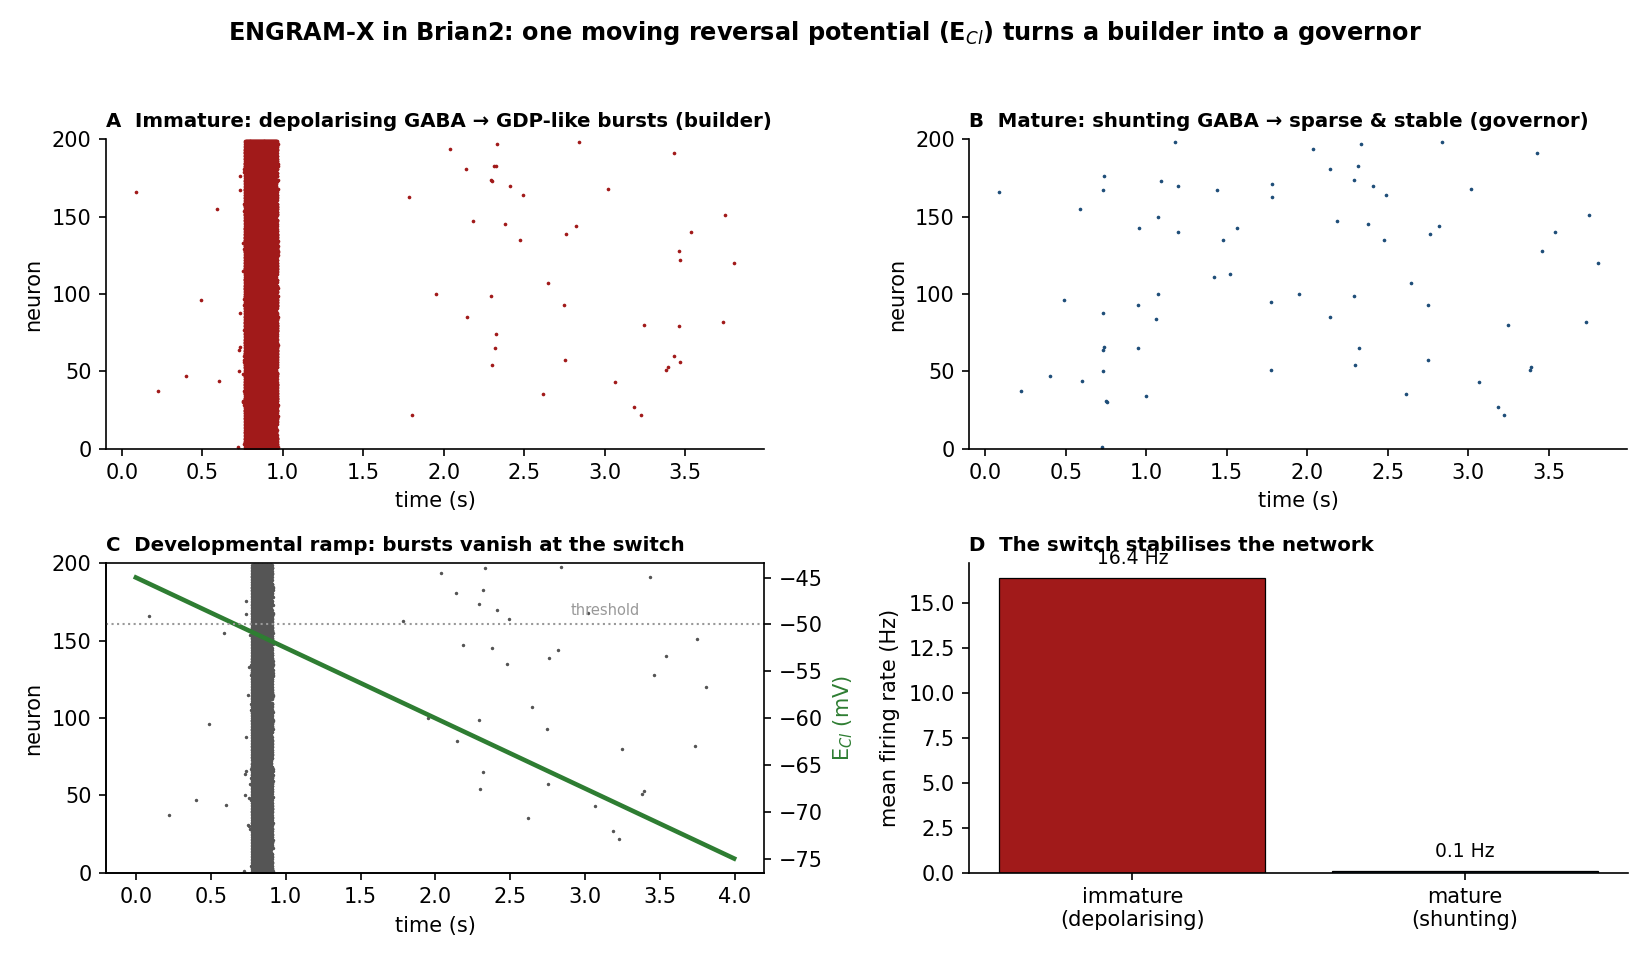
\includegraphics[width=0.9\linewidth]{demo_brian2_en.png}
\caption{\textbf{The GABA switch as a moving reversal potential (Brian2).} The same excitatory/inhibitory microcircuit at three chloride set points. (A) Immature, depolarizing GABA: synchronous, GDP-like discharges. (B) Mature, shunting GABA: sparse, stable activity. (C) A developmental $\ECl$ ramp: the discharges disappear as the reversal potential crosses threshold. (D) The mean firing rate collapses across the switch. Only $\ECl$ differs between conditions.}
\label{fig:sim}
\end{figure}

\subsection{Growing the XOR-like read-out: the coincidence-suppression core}\label{app:growth}
Correlation-based growth cannot carve XOR: ``those that fire together wire together'' reinforces coincidence, whereas XOR must \emph{suppress} it. The symmetry breaking is supplied instead by the switch, through the calcium-dependent plasticity of \S\ref{app:bg}(iv). An earlier version of this test held $\ECl$ fixed at rest, so the hub shunted from the start --- which cannot test a hypothesis that is about the \emph{transition}. Here $\ECl$ \emph{moves}. We build the circuit in Brian2: two Poisson inputs, two lateral principal cells, a pre-positioned set of inhibitory hub neurons (fixed, broadly connected, shunting only the laterals --- not the read-out, in keeping with Fig.~\ref{fig:mature}), and a read-out; only the direct input$\to$lateral arms are plastic.

The arms start \emph{below} the firing ``cliff'' ($w_0=0.10$, cliff $\approx0.21$), where the \emph{mean} single-input drive is subthreshold: a lateral spikes only rarely (at most a few hertz, from chance Poisson clusters), calcium is near zero, and plasticity is negligible on its own, so the arms cannot bootstrap unaided. The run has three phases: a \emph{builder} ($\ECl=-40$~mV, GABA depolarizing), a \emph{switch} ($\ECl$ ramps $-40\to-65$~mV over $5$~s), and a \emph{governor} ($\ECl=-65$~mV, GABA shunting). This removes the assumption the earlier hand-tuned rule required --- that the arms begin \emph{above} the cliff. Here the builder \emph{produces} that condition: while GABA is depolarizing the hub coactivates the laterals in GDP-like bursts that carry calcium and lift the arms over the cliff; the switch then converts the hub to shunting; and the grown, now supra-threshold arms are used by the governor to compute XOR. When one input is active its lateral escapes the shunt, gains high calcium and \emph{potentiates}; during coincidence the doubled shunt clamps the lateral, calcium collapses, and the arm \emph{depresses}. The shunt is at once the mature operation \emph{and} the teaching signal.

Each plastic arm $w$ (input$\to$lateral) follows a BCM sliding-threshold rule, updated every $\Delta t=1$~ms:
\begin{equation}
\Delta w \;=\; \eta\,x\,c\,(c-\theta),\qquad w \leftarrow \mathrm{clip}(w,\,w_{\min},\,w_{\max}),
\end{equation}
where $x$ is a presynaptic eligibility trace ($\dot{x}=-x/\tau_{\mathrm{pre}}$, $+1$ per presynaptic spike, $\tau_{\mathrm{pre}}=15$~ms); $c=\mathrm{Ca}/\kappa$ is a postsynaptic calcium proxy ($\dot{\mathrm{Ca}}=-\mathrm{Ca}/\tau_{\mathrm{Ca}}$, $+1$ per postsynaptic spike, $\tau_{\mathrm{Ca}}=60$~ms, $\kappa=9$); $\theta$ is the sliding threshold ($\dot{\theta}=(c^{2}-\theta)/\tau_{\theta}$, $\tau_{\theta}=800$~ms); $\eta=3\times10^{-5}$; and the weights are clipped to $[w_{\min},w_{\max}]=[0.05,2.6]$, with no explicit decay term (when $c=0$ the rule gives $\Delta w=0$).

Two details matter. First, the laterals carry a spike-frequency \emph{adaptation} current: without it, depolarizing GABA clamps a lateral at $\ECl=-40$~mV and it fires tonically at saturation, which drives $\theta=\langle c^{2}\rangle$ \emph{above} $c$, flips the sign of $(c-\theta)$, and makes the builder \emph{depress} the arms it should grow. Adaptation makes the depolarizing phase self-terminate into brief, high-calcium \emph{bursts} separated by quiet gaps --- exactly what giant depolarizing potentials are --- keeping $c>\theta$ so potentiation persists; the GDP structure is thus what lets the builder teach. Second, the test is hardened against artefacts: the hub cells carry \emph{heterogeneous} firing thresholds, so the bursts do not depend on artificial synchrony, and every probe follows a clean reset of all dynamic state, so residual adaptation cannot leak in.

\begin{figure}[h]
\centering

\includegraphics[width=0.86\linewidth]{phase_trace_en.png}
\caption{\textbf{The builder grows the arms; the governor uses them (Brian2, full sequence).} $\ECl$ (top) is depolarizing in the builder phase, ramps through the switch, and rests in the governor phase. The two direct input arms (bottom) start at $w_0=0.10$, \emph{below} the firing cliff (dashed): while GABA is depolarizing the hub coactivates the laterals in GDP-like bursts that carry calcium and lift the arms over the cliff; after the switch the grown, supra-threshold arms are used by the shunting governor to compute XOR. Without the builder the arms never leave $0.10$.}
\label{fig:trace}
\end{figure}

The developmental sequence is \emph{necessary}, not decorative, and a factorial set of controls shows it (Fig.~\ref{fig:factorial}). With the shunt mature from the start (no builder), or with no hub at all, the laterals never fire and the arms stay at $0.10$ --- \emph{collapse}. Running the \emph{same} $\ECl$ transition with plasticity frozen ($\eta=0$) collapses too, so the transition alone builds nothing: it is the plasticity, gated by the moving shunt, that carves the circuit. A builder that never switches off over-reinforces coincidence and gives \emph{OR}. Only the full builder$\to$switch$\to$governor sequence gives \emph{XOR}, a single input driving the read-out several times harder than coincidence. A direct \emph{arm-acquisition} test --- probing single inputs with the hub silenced --- confirms the developmental claim: after the full sequence \emph{both} arms fire on their own, so the builder lifted them over threshold, whereas after any collapse condition \emph{neither} arm has grown. Equivalently, probed \emph{before} any training the circuit collapses, and only \emph{after} the full sequence does it compute XOR --- the sequence, not either endpoint alone, creates the circuit.

\begin{figure}[h]
\centering

\includegraphics[width=\linewidth]{phase_factorial_en.png}
\caption{\textbf{Each developmental phase --- and plasticity itself --- is necessary (Brian2; arms start below the cliff, $w_0=0.1$; heterogeneous hub; clean reset before probing).} Read-out rates for the four input patterns ($10,01,11,00$) after training, under five manipulations. \emph{Governor only}, \emph{no hub}, and \emph{no plasticity} ($\eta=0$: the full $\ECl$ transition with learning frozen) $\to$ collapse (arms stay at $0.1$). \emph{Builder only} (the switch never happens) $\to$ OR (coincidence, $11$, is largest). \emph{Full sequence} $\to$ XOR. Beneath each panel: the trained arm weights and an \emph{arm-acquisition} verdict (single inputs probed with the hub silenced) --- ``both grown'' only where the builder ran, ``neither grown'' in every collapse case.}
\label{fig:factorial}
\end{figure}

Finally, the \emph{timing} of the switch matters (Fig.~\ref{fig:window}): too short a builder and the arms never clear the cliff (collapse); too long and the builder over-grows them until the mature shunt can no longer suppress coincidence (OR, the limit approached by the never-switching control). A hardened spot-check (heterogeneous hub) places the lower, collapse boundary firmly near $t_{\mathrm{build}}\approx10$~s, with XOR robust from there through very long builders; the upper, OR boundary sits much later than an earlier correlated-hub sweep suggested, because artificial hub synchrony exaggerated the over-growth. The developmental window is therefore real and \emph{firm on its early edge}, softer on its late edge: advancing the switch robustly predicts collapse, delaying it eventually predicts loss of selectivity.

\begin{figure}[h]
\centering

\includegraphics[width=0.72\linewidth]{window2d_en.png}
\caption{\textbf{A developmental window for the switch (Brian2 sweep, 3 seeds per cell).} Outcome of the full two-phase model as the builder duration $t_{\mathrm{build}}$ (when the switch happens) is swept against the mature shunt strength; each cell gives the majority class, the vote, and the mean single/coincidence read-out rate (Hz). XOR (green) occupies a broad contiguous band, bounded below by collapse (switch too early) and above by OR (switch too late). \emph{This sweep used the earlier correlated-hub code}; a hardened, heterogeneous-hub spot-check confirms the collapse boundary and the XOR interior but places the OR boundary at substantially longer builder durations (see text). Developmental timing is a parameter with an interior optimum.}
\label{fig:window}
\end{figure}

\textbf{Robustness across seeds, and the role of hub correlation.} Because a single run cannot support a developmental-learning claim, we repeated the full sequence over $100$ random seeds and classified \emph{each} run individually (Fig.~\ref{fig:robust}). With the shared-input hub the outcome is effectively deterministic: XOR in $100/100$ runs, both arms grown in $100/100$, median $\mathrm{xor\_index}=0.78$ (IQR $[0.70,0.81]$), coincidence held to $R_{11}=8$~Hz (IQR $[8,11]$) against single-input rates of ${\sim}41$~Hz; a fully-random (unbalanced) pattern-exposure control is essentially identical (XOR $96/100$; the four exceptions are borderline sub-threshold single-input rates that remain XOR-like by the continuous index), so the result is not an artefact of balanced exposure. The one manipulation that does matter is the correlation of the hub's afferents: when each hub cell receives a mixture of the shared trains and its own independent, pattern-driven train, coincidence suppression degrades smoothly as sharing is reduced --- $R_{11}$ rises monotonically ($8\to87$~Hz), $\mathrm{xor\_index}$ falls and crosses zero near $\mathrm{shared}\approx0.66$, and the XOR fraction drops through a knee near $0.82$, becoming OR by $\mathrm{shared}\leq0.6$. Crucially, \emph{both arms grow in $100\%$ of runs across the entire sweep}: what fails as the hub de-correlates is not the growth of the direct arms but the coincidence-dependent shunt. This sharpens what the model shows --- the plasticity does not discover the XOR architecture, which is preconfigured (both inputs onto the hub, the hub's supralinear threshold, the hub onto both laterals, the read-out pooling both laterals, mature GABA shunting); rather, the two-phase sequence \emph{matures} it, the depolarizing builder lifting otherwise-subthreshold arms into a functional regime and the switch then letting the same pre-positioned hub express coincidence suppression, \emph{provided} that suppression rests on the synchronous recruitment of a correlated hub population.

\begin{figure}[h]
\centering
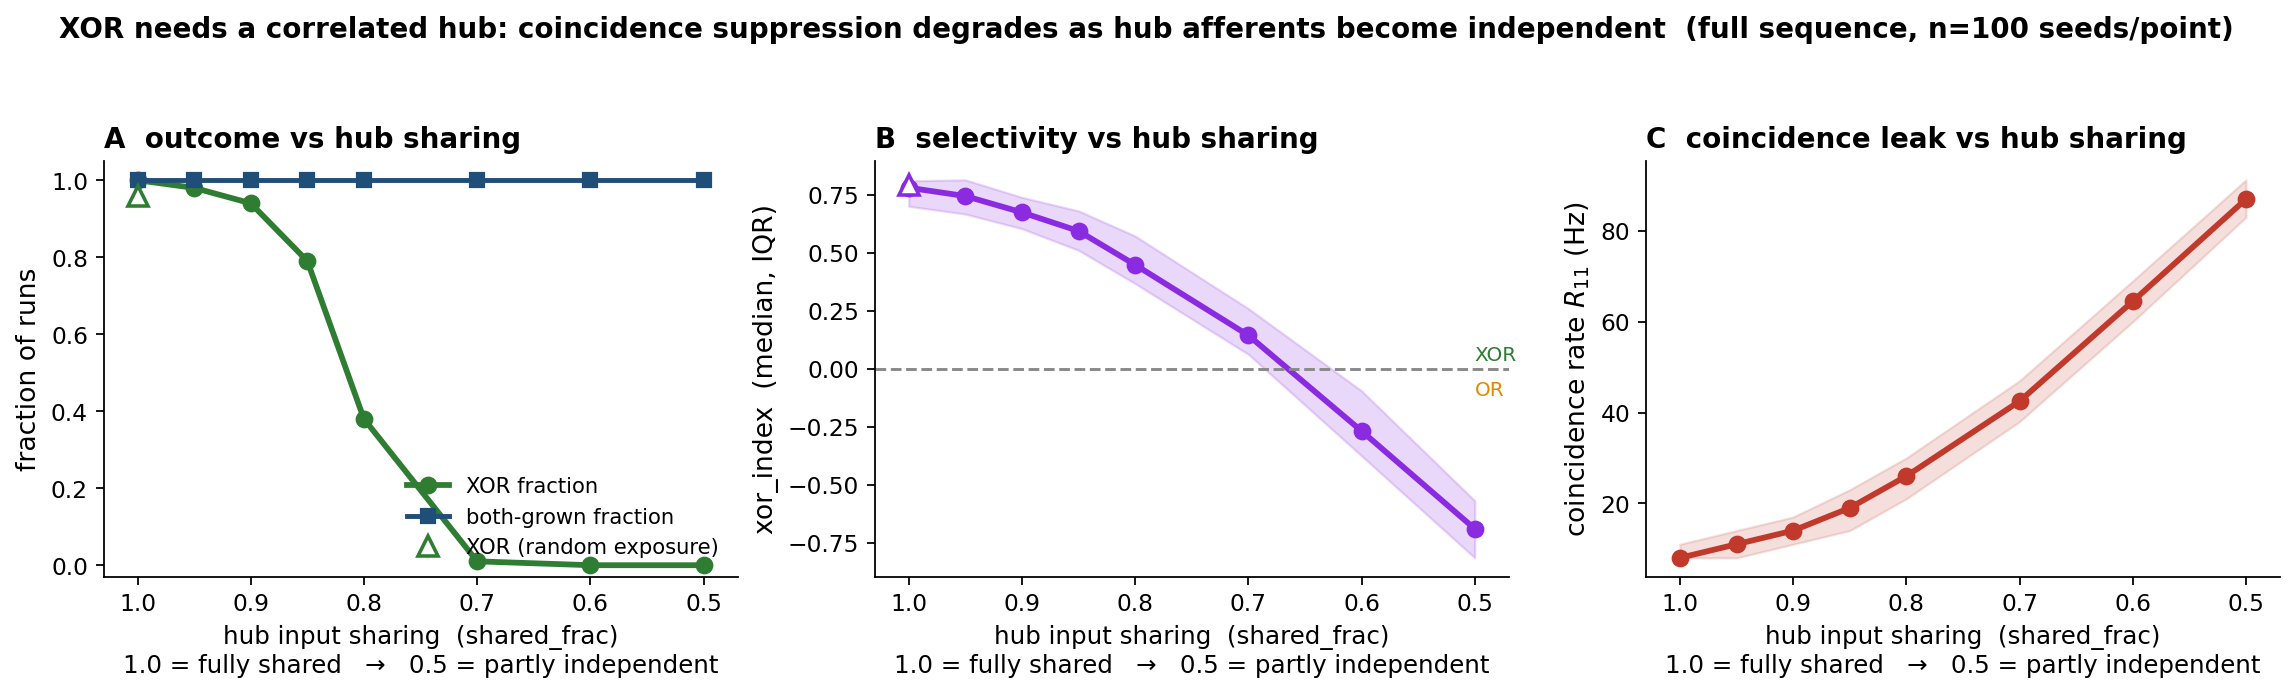
\includegraphics[width=\linewidth]{robustness_sweep_en.png}
\caption{\textbf{XOR requires a correlated hub (Brian2, 100 seeds per point).} As the fraction of \emph{shared} afferent drive to the 20 hub cells falls from 1.0 (all hubs see the same two Poisson trains) towards 0.5 (each hub also receives its own independent, pattern-driven train), coincidence suppression degrades smoothly. \textbf{(A)} the fraction of runs classified XOR falls from $1.00$ through a knee near $\mathrm{shared}\!\approx\!0.82$, while the fraction in which \emph{both} direct arms grew stays at $1.00$ throughout. \textbf{(B)} the continuous selectivity index $\mathrm{xor\_index}=(\min(R_{10},R_{01})-R_{11})/\min(R_{10},R_{01})$ (median, IQR band) declines monotonically and crosses zero (XOR$\to$OR) near $\mathrm{shared}\!\approx\!0.66$. \textbf{(C)} the coincidence read-out rate $R_{11}$ rises from ${\sim}8$ to ${\sim}87$~Hz. Open triangles: a fully-random (unbalanced) pattern-exposure control at $\mathrm{shared}=1.0$ (XOR $0.96$), confirming the result does not depend on balanced exposure.}
\label{fig:robust}
\end{figure}

Honest limits: the emergent XOR is clean and symmetric but \emph{soft} (coincidence held to a fraction of the single-input rate, not annihilated); the grown circuit sits in a low-rate regime; and the plasticity rule, though BCM-grounded, is a stylized abstraction, not a fit to measured plasticity. Both simulations and every figure script are in the code repository (Data and code, main text).


\FloatBarrier
\section{The GABA switch in the hippocampus}\label{app:hipp}
In the mammalian hippocampus the switch is elaborated into a developmental \emph{programme}, and it is here that its constructive role is clearest. Inhibition is built first: GABAergic neurons and their synapses appear before glutamatergic ones, and in the immature network GABA is depolarizing and, under the right conditions, excitatory (Ben-Ari, 2002; Ben-Ari et al., 2007). The molecular cause is the late induction of the neuron-specific chloride extruder KCC2, which lowers $[\Clm]_{\mathrm{in}}$ and renders GABA hyperpolarizing as neurons mature; suppressing KCC2 shifts the GABA reversal potential back towards depolarizing values (Rivera et al., 1999).

While it remains depolarizing, GABA does not merely coexist with development --- it \emph{drives} it. Immature GABA generates Giant Depolarizing Potentials (GDPs), the first coordinated network activity of the hippocampus (Ben-Ari et al., 1989), produced by the synergistic excitatory action of GABA$_{\mathrm{A}}$ and NMDA receptors and accompanied by the calcium transients that guide the growth and stabilization of synapses (Leinekugel et al., 1997). These events are orchestrated by a small population of richly connected GABAergic \emph{hub} interneurons, whose wide axonal fields pace the synchrony; stimulating a single hub can advance, delay, or abort a GDP across the whole network (Bonifazi et al., 2009; Cossart \& Khazipov, 2022). The picture is that of a common inhibitory hub which, in its depolarizing phase, coactivates and so helps to \emph{grow} the very excitatory arms it will later regulate.

The decisive subtlety is that the inhibitory \emph{conductance} is present the whole time; only the \emph{sign of its driving force} changes. As KCC2 rises and $\ECl$ falls towards rest, the same hub stops depolarizing and begins to \emph{shunt} --- the divisive, gain-controlling operation described in the biophysical background (Appendix~\ref{app:sim}). One topology; two computational modes, selected by a slow chloride set point (Fig.~\ref{fig:dev}; the circuit itself, in its builder and governor forms, is Fig.~\ref{fig:devseq}A,C). And because KCC2 expression is itself activity-dependent, the switch is a homeostatic negative feedback that moves the network out of its highly synchronous GDP regime towards the sparse, marginally stable operating point of the adult.

\begin{figure}[h]
\centering
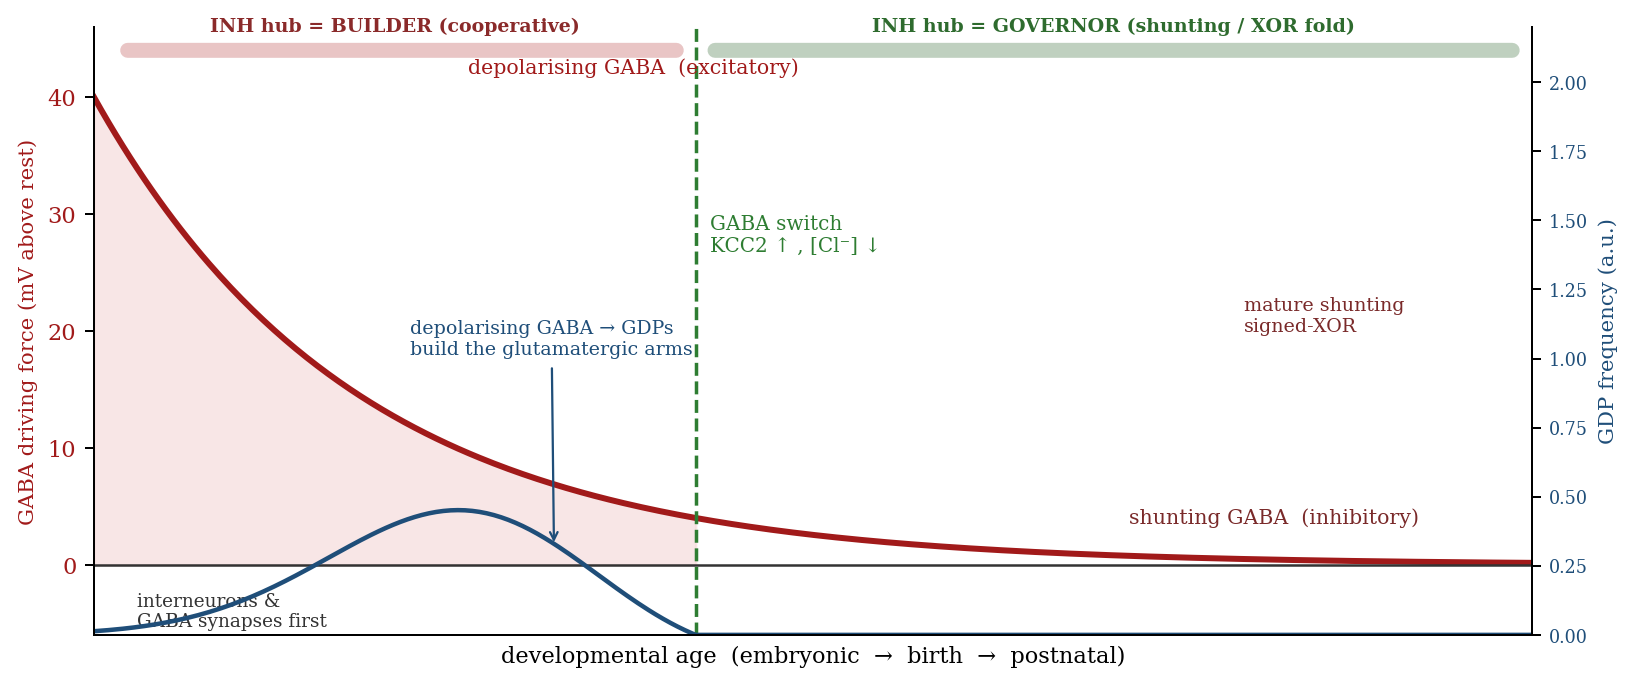
\includegraphics[width=0.92\linewidth]{preprint_fig_en.png}
\caption{\textbf{The builder$\rightarrow$governor hypothesis.} Early in the development the GABA driving force is strongly depolarizing (red); the inhibitory hub acts cooperatively and paces the giant depolarizing potentials (blue), whose calcium transients grow the glutamatergic arms of the circuit. As KCC2 rises and intracellular chloride falls (the ``GABA switch''), the driving force collapses towards rest, the GDPs disappear, and the same hub becomes a shunting governor into which the mature signed-XOR read-out is folded. One topology; two computational modes, selected by a slow chloride set point. Schematic; axes illustrative.}
\label{fig:dev}
\end{figure}

\FloatBarrier
\section{The GABA switch in \emph{C.~elegans}}\label{app:worm}
The developmental GABA switch, once considered a vertebrate peculiarity, reaches down to the nematode. In the locomotor circuit of \emph{C.~elegans}, the GABA$_{\mathrm{A}}$ agonist muscimol \emph{excites} muscle in newly hatched (L1) animals and, by the middle of the first larval stage (about six hours after hatching), \emph{relaxes} it --- a reversal from depolarizing to hyperpolarizing. The switch runs on the same chloride machinery as in mammals: the importer NKCC-1 sustains the early depolarizing response, while the extruders KCC-2 and ABTS-1 produce the later hyperpolarizing one. Tellingly, the switch still occurs (with a delay) in \emph{unc-25} mutants that cannot synthesize GABA at all, showing that in the worm it is largely a \emph{cell-intrinsic, programmed} maturation of the chloride gradient rather than something driven by neural activity (Han et al., 2015). The extruders were characterized independently: KCC-2 sets the chloride gradients required for inhibition, is upregulated during synaptic development, and operates in both neurons and muscle (Tanis et al., 2009); it acts together with ABTS-1, and when both are removed the gradient reverses so that GABA excites rather than inhibits (Bellemer et al., 2011).

A very recent result carries the depolarizing phase down to the embryo. Immature GABAergic DD motor neurons transiently inhibit early embryonic movement, about 8.5--9.5 hours after fertilization, \emph{before} their neurites have finished growing and before most of the nerve-ring synapses exist; the effect requires GABA synthesis in the DD neurons and UNC-49 GABA$_{\mathrm{A}}$ receptors in the muscle, occurs through both synaptic and non-synaptic (tonic) release, and follows chloride logic --- removing the importer NKCC-1 deepens the inhibition while removing the extruder KCC-2 relieves it (Marvel-Coen et al., 2026). The chloride-controlled sign of GABA is thus in place from the embryo onwards.

Two complications refine, rather than break, the picture. The worm has a \emph{second} route to an excitatory GABA that bypasses the chloride gradient entirely: EXP-1 is a GABA-gated cation channel, excitatory by construction (Beg \& Jorgensen, 2003), showing that the sign of a ``GABA'' signal can be set either by the transporter-controlled driving force or intrinsically by the receptor. And although eight connectomes have already been reconstructed across postembryonic development --- revealing a largely constant wiring scaffold that becomes progressively more feedforward with age (Witvliet et al., 2021) --- connectomes report anatomy, not $\ECl$, and the ``builder'' depolarizing phase is largely embryonic. The worm establishes that the switch is conserved and cell-intrinsic; it does not, on its own, show the switch operating inside a central computational circuit. That is where the mammalian data (Appendix~\ref{app:hipp}) go further.

\FloatBarrier
\section{Chloride and GABA in plants}\label{app:plants}
A caveat, on which the main text also insists, comes before drawing the parallel: what follows is a claim of \emph{functional repurposing}, not of homology --- the plant and animal proteins are unrelated, and all that is shared is the ancient \emph{principle} of ion control and the cotransporter family that implements it.

Long before neurons, cells used chloride to move. Chloride is the most abundant inorganic anion in plant cells and, though long dismissed as a mere micronutrient, it accumulates to osmotically decisive concentrations and is today recognized as a beneficial macronutrient, central to osmoregulation and turgor (Geilfus, 2018; Colmenero-Flores et al., 2019). The direction is what matters: plant cells keep $[\Clm]_{\mathrm{in}}$ \emph{high}, because in a walled cell a high internal osmolyte is what generates the turgor pressure that drives growth and movement --- exactly the opposite of the mature neuron, which spends energy to keep $[\Clm]_{\mathrm{in}}$ \emph{low}.

Because turgor is the plant's actuator, chloride is the plant currency of movement. The opening and closing of stomata is a turgor motor in which anion channels are the active elements: the malate-activated vacuolar channel AtALMT9 is required for opening, and the R-type channel AtALMT12/QUAC1 mediates the anionic efflux of closure (De Angeli et al., 2013; Meyer et al., 2010). Faster movements use the same anions as a genuine excitable system: the Venus flytrap fires an all-or-none action potential carried by a calcium-activated \emph{anionic} conductance rather than a sodium current, and even \emph{counts} those action potentials to commit to digestion (B\"ohm et al., 2016). Plants even use GABA as a signal, but through a different protein and with the sign reversed: GABA regulates the ALMT anion channels, which are \emph{not} homologous to the animal GABA$_{\mathrm{A}}$ receptor (they share only a $\sim$12-amino-acid motif; Ramesh et al., 2015, 2017, 2018), and because the internal anions are high, opening an ALMT channel \emph{depolarizes} while GABA, by \emph{closing} it, hyperpolarizes.

Do plants have the switch itself? They have the machinery family but not the neuronal specialization. Cation-chloride cotransporters exist in plants, but flowering plants typically carry a single such gene (\emph{AtCCC} in Arabidopsis), phylogenetically closest to the KCC clade and yet localized largely to endomembranes and the vasculature, and not deployed as a plasma-membrane extruder that sets a resting $\ECl$ for inhibition (Colmenero-Flores et al., 2007; Henderson et al., 2018). Plants therefore possess every ancient ingredient --- chloride, anion channels, GABA, cotransporters --- but not the diversified extrusion switch, and their chloride ``default'' points in the wrong direction for inhibition. That missing switch is exactly what the animal lineage adds, and it is where movement becomes control.

\FloatBarrier
\section*{References}
\small
\begin{apabib}
\item Beg, A.~A., \& Jorgensen, E.~M. (2003). EXP-1 is an excitatory GABA-gated cation channel. \emph{Nature Neuroscience, 6}(11), 1145--1152. \url{https://doi.org/10.1038/nn1136}
\item Beggs, J.~M., \& Plenz, D. (2003). Neuronal avalanches in neocortical circuits. \emph{Journal of Neuroscience, 23}(35), 11167--11177. \url{https://doi.org/10.1523/JNEUROSCI.23-35-11167.2003}
\item Bellemer, A., Hirata, T., Romero, M.~F., \& Koelle, M.~R. (2011). Two types of chloride transporters are required for GABA$_{\mathrm{A}}$ receptor-mediated inhibition in \emph{C.~elegans}. \emph{The EMBO Journal, 30}(9), 1852--1863. \url{https://doi.org/10.1038/emboj.2011.83}
\item Ben-Ari, Y. (2002). Excitatory actions of GABA during development: the nature of the nurture. \emph{Nature Reviews Neuroscience, 3}(9), 728--739. \url{https://doi.org/10.1038/nrn920}
\item Ben-Ari, Y., Cherubini, E., Corradetti, R., \& Gaiarsa, J.-L. (1989). Giant synaptic potentials in immature rat CA3 hippocampal neurones. \emph{The Journal of Physiology, 416}, 303--325. \url{https://doi.org/10.1113/jphysiol.1989.sp017762}
\item Ben-Ari, Y., Gaiarsa, J.-L., Tyzio, R., \& Khazipov, R. (2007). GABA: a pioneer transmitter that excites immature neurons and generates primitive oscillations. \emph{Physiological Reviews, 87}(4), 1215--1284. \url{https://doi.org/10.1152/physrev.00017.2006}
\item Bienenstock, E.~L., Cooper, L.~N., \& Munro, P.~W. (1982). Theory for the development of neuron selectivity: orientation specificity and binocular interaction in visual cortex. \emph{Journal of Neuroscience, 2}(1), 32--48. \url{https://doi.org/10.1523/JNEUROSCI.02-01-00032.1982}
\item B\"ohm, J., Scherzer, S., Krol, E., Kreuzer, I., von Meyer, K., Lorey, C., \ldots\ Hedrich, R. (2016). The Venus flytrap \emph{Dionaea muscipula} counts prey-induced action potentials to induce sodium uptake. \emph{Current Biology, 26}(3), 286--295. \url{https://doi.org/10.1016/j.cub.2015.11.057}
\item Bonifazi, P., Goldin, M., Picardo, M.~A., Jorquera, I., Cattani, A., Bianconi, G., Represa, A., Ben-Ari, Y., \& Cossart, R. (2009). GABAergic hub neurons orchestrate synchrony in developing hippocampal networks. \emph{Science, 326}(5958), 1419--1424. \url{https://doi.org/10.1126/science.1175509}
\item Carandini, M., \& Heeger, D.~J. (2012). Normalization as a canonical neural computation. \emph{Nature Reviews Neuroscience, 13}(1), 51--62. \url{https://doi.org/10.1038/nrn3136}
\item Clopath, C., B\"using, L., Vasilaki, E., \& Gerstner, W. (2010). Connectivity reflects coding: a model of voltage-based STDP with homeostasis. \emph{Nature Neuroscience, 13}(3), 344--352. \url{https://doi.org/10.1038/nn.2479}
\item Colmenero-Flores, J.~M., Mart\'inez, G., Gamba, G., V\'azquez, N., Iglesias, D.~J., Brum\'os, J., \& Tal\'on, M. (2007). Identification and functional characterization of cation--chloride cotransporters in plants. \emph{The Plant Journal, 50}(2), 278--292. \url{https://doi.org/10.1111/j.1365-313X.2007.03048.x}
\item Colmenero-Flores, J.~M., Franco-Navarro, J.~D., Cubero-Font, P., Peinado-Torrubia, P., \& Rosales, M.~A. (2019). Chloride as a beneficial macronutrient in higher plants. \emph{International Journal of Molecular Sciences, 20}(19), 4686. \url{https://doi.org/10.3390/ijms20194686}
\item Cossart, R., \& Khazipov, R. (2022). How development sculpts hippocampal circuits and function. \emph{Physiological Reviews, 102}(1), 343--378. \url{https://doi.org/10.1152/physrev.00044.2020}
\item De Angeli, A., Zhang, J., Meyer, S., \& Martinoia, E. (2013). AtALMT9 is a malate-activated vacuolar chloride channel required for stomatal opening in Arabidopsis. \emph{Nature Communications, 4}, 1804. \url{https://doi.org/10.1038/ncomms2815}
\item Friedel, P., Kahle, K.~T., Zhang, J., Hertz, N., Pisella, L.~I., Buhler, E., Schaller, F., Duan, J., Khanna, A.~R., Bishop, P.~N., Shokat, K.~M., \& Medina, I. (2015). WNK1-regulated inhibitory phosphorylation of the KCC2 cotransporter maintains the depolarizing action of GABA in immature neurons. \emph{Science Signaling, 8}(383), ra65. \url{https://doi.org/10.1126/scisignal.aaa0354}
\item Geilfus, C.-M. (2018). Chloride: from nutrient to toxicant. \emph{Plant and Cell Physiology, 59}(5), 877--886. \url{https://doi.org/10.1093/pcp/pcy071}
\item Graupner, M., \& Brunel, N. (2012). Calcium-based plasticity model explains sensitivity of synaptic changes to spike pattern, rate, and dendritic location. \emph{Proceedings of the National Academy of Sciences, 109}(10), 3991--3996. \url{https://doi.org/10.1073/pnas.1109359109}
\item Han, B., Bellemer, A., \& Koelle, M.~R. (2015). An evolutionarily conserved switch in response to GABA affects development and behavior of the locomotor circuit of \emph{Caenorhabditis elegans}. \emph{Genetics, 199}(4), 1159--1172. \url{https://doi.org/10.1534/genetics.114.173963}
\item Hartmann, A.-M., Tesch, D., Nothwang, H.~G., \& Bininda-Emonds, O.~R.~P. (2014). Evolution of the cation chloride cotransporter family: ancient origins, gene losses, and subfunctionalization through duplication. \emph{Molecular Biology and Evolution, 31}(2), 434--447. \url{https://doi.org/10.1093/molbev/mst225}
\item Henderson, S.~W., Wege, S., \& Gilliham, M. (2018). Plant cation-chloride cotransporters (CCC): evolutionary origins and functional insights. \emph{International Journal of Molecular Sciences, 19}(2), 492. \url{https://doi.org/10.3390/ijms19020492}
\item J\'ekely, G., Keijzer, F., \& Godfrey-Smith, P. (2015). An option space for early neural evolution. \emph{Philosophical Transactions of the Royal Society B, 370}(1684), 20150181. \url{https://doi.org/10.1098/rstb.2015.0181}
\item Keijzer, F., van Duijn, M., \& Lyon, P. (2013). What nervous systems do: early evolution, input--output, and the skin brain thesis. \emph{Adaptive Behavior, 21}(2), 67--85. \url{https://doi.org/10.1177/1059712312465330}
\item Leinekugel, X., Medina, I., Khalilov, I., Ben-Ari, Y., \& Khazipov, R. (1997). Ca$^{2+}$ oscillations mediated by the synergistic excitatory actions of GABA$_{\mathrm{A}}$ and NMDA receptors in the neonatal hippocampus. \emph{Neuron, 18}(2), 243--255. \url{https://doi.org/10.1016/S0896-6273(00)80265-2}
\item Ma, Z., Turrigiano, G.~G., Wessel, R., \& Hengen, K.~B. (2019). Cortical circuit dynamics are homeostatically tuned to criticality in vivo. \emph{Neuron, 104}(4), 655--664.e4. \url{https://doi.org/10.1016/j.neuron.2019.08.031}
\item Marco de Lucas, J. (2024). From worms to mice: homeostasis maybe all you need. \emph{arXiv}. \url{https://arxiv.org/abs/2412.20090}
\item Marco de Lucas, J., Pe\~na Fern\'andez, M., \& Lloret Iglesias, L. (2024). Implementing engrams from a machine learning perspective: XOR as a basic motif. \emph{arXiv}. \url{https://arxiv.org/abs/2406.09940}
\item Marco de Lucas, J., Pe\~na Fern\'andez, M., \& Lloret Iglesias, L. (2026). \emph{Signed XOR feedback} (European Patent Application No.~26382252.0). European Patent Office.
\item Marvel-Coen, J., Ardiel, E., Zhao, J., Nurrish, S., \& Kaplan, J.~M. (2026). Immature \emph{Caenorhabditis elegans} motor neurons control early embryo behavior via both synaptic and nonsynaptic GABA release. \emph{Proceedings of the National Academy of Sciences, 123}(2), e2508541123. \url{https://doi.org/10.1073/pnas.2508541123}
\item Meyer, S., Mumm, P., Imes, D., Endler, A., Weder, B., Al-Rasheid, K.~A.~S., \ldots\ Hedrich, R. (2010). AtALMT12 represents an R-type anion channel required for stomatal movement in Arabidopsis guard cells. \emph{The Plant Journal, 63}(6), 1054--1062. \url{https://doi.org/10.1111/j.1365-313X.2010.04302.x}
\item Moroz, L.~L., Kocot, K.~M., Citarella, M.~R., Dosung, S., Norekian, T.~P., Povolotskaya, I.~S., \ldots\ Kohn, A.~B. (2014). The ctenophore genome and the evolutionary origins of neural systems. \emph{Nature, 510}(7503), 109--114. \url{https://doi.org/10.1038/nature13400}
\item Pe\~na Fern\'andez, M., Gonz\'alez R\'ios, A., Lloret Iglesias, L., \& Marco de Lucas, J. (2026a). From homeostasis to credit assignment: a signed-XOR connectomic motif for local directional error signalling. \emph{bioRxiv}. \url{https://doi.org/10.64898/2026.06.05.730322}
\item Pe\~na Fern\'andez, M., Lloret Iglesias, L., \& Marco de Lucas, J. (2026b). Toward defining loss functions in neuroscience: an XOR-based neuronal mechanism. \emph{bioRxiv}. \url{https://doi.org/10.64898/2026.03.16.712061}
\item Pe\~na Fern\'andez, M., Lloret Iglesias, L., \& Marco de Lucas, J. (2026c). Signed-XOR error and sparse coding in a Dale-compliant substrate for sequence memorization. \emph{bioRxiv}. \url{https://doi.org/10.64898/2026.06.24.734176}
\item Piala, A.~T., Moon, T.~M., Akella, R., He, H., Cobb, M.~H., \& Goldsmith, E.~J. (2014). Chloride sensing by WNK1 involves inhibition of autophosphorylation. \emph{Science Signaling, 7}(324), ra41. \url{https://doi.org/10.1126/scisignal.2005050}
\item Ramesh, S.~A., Tyerman, S.~D., Xu, B., Bose, J., Kaur, S., Conn, V., \ldots\ Gilliham, M. (2015). GABA signalling modulates plant growth by directly regulating the activity of plant-specific anion transporters. \emph{Nature Communications, 6}, 7879. \url{https://doi.org/10.1038/ncomms8879}
\item Ramesh, S.~A., Tyerman, S.~D., Gilliham, M., \& Xu, B. (2017). $\gamma$-Aminobutyric acid (GABA) signalling in plants. \emph{Cellular and Molecular Life Sciences, 74}(9), 1577--1603. \url{https://doi.org/10.1007/s00018-016-2415-7}
\item Ramesh, S.~A., Kamran, M., Sullivan, W., Chirkova, L., Okamoto, M., Degryse, F., McLaughlin, M., Gilliham, M., \& Tyerman, S.~D. (2018). Aluminum-activated malate transporters can facilitate GABA transport. \emph{The Plant Cell, 30}(5), 1147--1164. \url{https://doi.org/10.1105/tpc.17.00864}
\item Rinehart, J., Maksimova, Y.~D., Tanis, J.~E., Stone, K.~L., Hodson, C.~A., Zhang, J., Risinger, M., Pan, W., Wu, D., Colangelo, C.~M., Forbush, B., Joiner, C.~H., Gulcicek, E.~E., Gallagher, P.~G., \& Lifton, R.~P. (2009). Sites of regulated phosphorylation that control K-Cl cotransporter activity. \emph{Cell, 138}(3), 525--536. \url{https://doi.org/10.1016/j.cell.2009.05.031}
\item Rivera, C., Voipio, J., Payne, J.~A., Ruusuvuori, E., Lahtinen, H., Lamsa, K., Pirvola, U., Saarma, M., \& Kaila, K. (1999). The K$^{+}$/Cl$^{-}$ co-transporter KCC2 renders GABA hyperpolarizing during neuronal maturation. \emph{Nature, 397}(6716), 251--255. \url{https://doi.org/10.1038/16697}
\item Scellier, B., \& Bengio, Y. (2017). Equilibrium propagation: bridging the gap between energy-based models and backpropagation. \emph{Frontiers in Computational Neuroscience, 11}, 24. \url{https://doi.org/10.3389/fncom.2017.00024}
\item Tanis, J.~E., Bellemer, A., Moresco, J.~J., Forbush, B., \& Koelle, M.~R. (2009). The potassium chloride cotransporter KCC-2 coordinates development of inhibitory neurotransmission and synapse structure in \emph{Caenorhabditis elegans}. \emph{Journal of Neuroscience, 29}(32), 9943--9954. \url{https://doi.org/10.1523/JNEUROSCI.1989-09.2009}
\item Turrigiano, G.~G. (2008). The self-tuning neuron: synaptic scaling of excitatory synapses. \emph{Cell, 135}(3), 422--435. \url{https://doi.org/10.1016/j.cell.2008.10.008}
\item Whittington, J.~C.~R., \& Bogacz, R. (2017). An approximation of the error backpropagation algorithm in a predictive coding network with local Hebbian synaptic plasticity. \emph{Neural Computation, 29}(5), 1229--1262. \url{https://doi.org/10.1162/NECO\_a\_00949}
\item Witvliet, D., Mulcahy, B., Mitchell, J.~K., Meirovitch, Y., Berger, D.~R., Wu, Y., \ldots\ Zhen, M. (2021). Connectomes across development reveal principles of brain maturation. \emph{Nature, 596}(7871), 257--261. \url{https://doi.org/10.1038/s41586-021-03778-8}
\end{apabib}

\end{document}
